\section{Software}
\label{sec:TeilB_Software}
Um die EDID-Daten in das EEPROM schreiben zu können, muss der Prozessor mit einer gewissen Software programmiert werden. Durch die Verbindung über die USB-Bridge kommuniziert der Prozessor mit dem Computer. Der Datenaustausch arbeitet nach einem definierten Protokoll, auf welches im Softwarekonzept eingegangen wird. Im Anschluss wird die Embedded- sowie die PC-Software mit ihren einzelnen Komponenten beschrieben. 
\subsection{Softwarekonzept}
\label{softwarekonzept}
Um mit dem Prozessor zu kommunizieren, stehen dem PC vier Kommandos zur Verfügung. Diese werden über die Serielle Schnittstelle vom Prozessor empfangen. Die Kommandos folgen dem Format \code{\#Kommando\*}. Sodass ein Kommando definiert von Anfang bis Ende empfangen werden kann, werden die Code-Zeichen \code{\#} und \code{\*} verwendet. Mit dem Zeichen \code{\#} wird dem Prozessor mitgeteilt, dass alle nachfolgenden Zeichen ein Kommando darstellen. Um das Ende des Kommandos mitzuteilen wird das Zeichne \code{\*} gesendet. Wird ein Kommando vollständig empfangen, so wird es interpretiert und die entsprechend Funktion aufgerufen. Nach erfolgreicher Ausführung der entsprechenden Funktion wird ein Return-Wert an den PC gesendet. Die verfügbaren Kommandos um mit dem Prozessor zu kommunizieren und deren Rückgabewerte sind in \reft{tab:avr_commands} beschriebenen.
\begin{table}[h]
\begin{tabular}{|p{6.5cm}|p{2.5cm}|p{3.5cm}|}\hline
\rowcolor{TableBackgroundColor} 
   \textbf{Beschreibung} & \textbf{Kommando} & \textbf{Rückgabewert}	\\ \hline
	Handshake empfangen & \#h* & keiner \\ \hline    
    Start des Schreibvorgangs und setze Adresse im EEPROM auf Null & \#s* & \#1* \\ \hline
    Inkrementiere Adresse im EEPROM und schreibe Daten& \#wX* & \#2* \\ \hline
    Beende Schreibvorgang & \#x* & \#3* \\ \hline
	Prüfsumme angefordert & \#c* & gibt aktuelle Prüfsumme zurück\\ \hline    
    Debug-Ausgabe & \#d* & gibt aktuellen EEPROM-Inhalt zurück\\ \hline
\end{tabular}
\caption{Kommandos zum Schreiben des EEPROMs}
\label{tab:avr_commands}
\end{table} \\
Ein Ablaufdiagramm der Funktionalität zum Beschreiben des EEPROMs ist in \refa{fig:ablaufdiagramm_avr} zu sehen. Nach dem Start des Prozessors sendet der ein Handshake \code{h}. Verbindet sich das PC-Prorammm mit der seriellen Schnittstelle und korrekter Baudrate, werden diese Aufforderungen zum Handshake empfangen. Die PC-Software antwortet ebenfalls mit \code{h}, was beiden Teilnehmern die Anwesenheit des anderen bestätigt. Der AVR\footnote{AVR: Atmel ATMEGA Prozessor, Akronym für: \textbf{A}lf (Egil Bogen) and \textbf{V}egard (Wollan)'s \textbf{R}ISC processor} ist somit Bereit zum Empfangen von Kommandos (siehe \reft{tab:avr_commands}). Um das EEPROM zu beschreiben, wird vom PC das Kommando \code{\#s\*} gesendet, was dem AVR mitteilt, dass im Folgenden Daten zum Beschreiben des EEPROMs gesendet werden. Der PC sendet nun 128 mal das Kommando \code{\#wX\*}, um die 128 Bytes der EDID-Informationen zu senden. Das \code{X} steht für einen Platzhalter und entspricht der Hexadezimalen Schreibweise für binäre Werte von 0 bis 255. Um dem AVR mitzuteilen, dass das Beschreiben des EEPROMs beendet werden und damit keine Daten mehr gesendet werden, wird das Kommando \code{\#x\*} gesendet. Nach jedem empfangenen Kommando sendet der AVR jeweils den Rückgabewert aus \reft{tab:avr_commands} für das entsprechende Kommando. Die PC-Software wartet auf den Empfang des Rückgabewerts und fährt erst nach Erhalt dessen mit dem Schreiben weiterer Kommandos fort. Nachdem alle Bytes in das EEPROM geschrieben sind, fordert das Programm mit \code{\#c\*} die Prüfsumme der EEPROM-Daten an. Dieser Schritt ist notwendig um die Integrität der Daten zu prüfen. Ist bei der Kommunikation ein Fehler unterlaufen, so unterscheiden sich die beiden Prüfsummen von EEPROM und PC-Programm.\\
\begin{figure}[htp]
	\center
	\fbox{	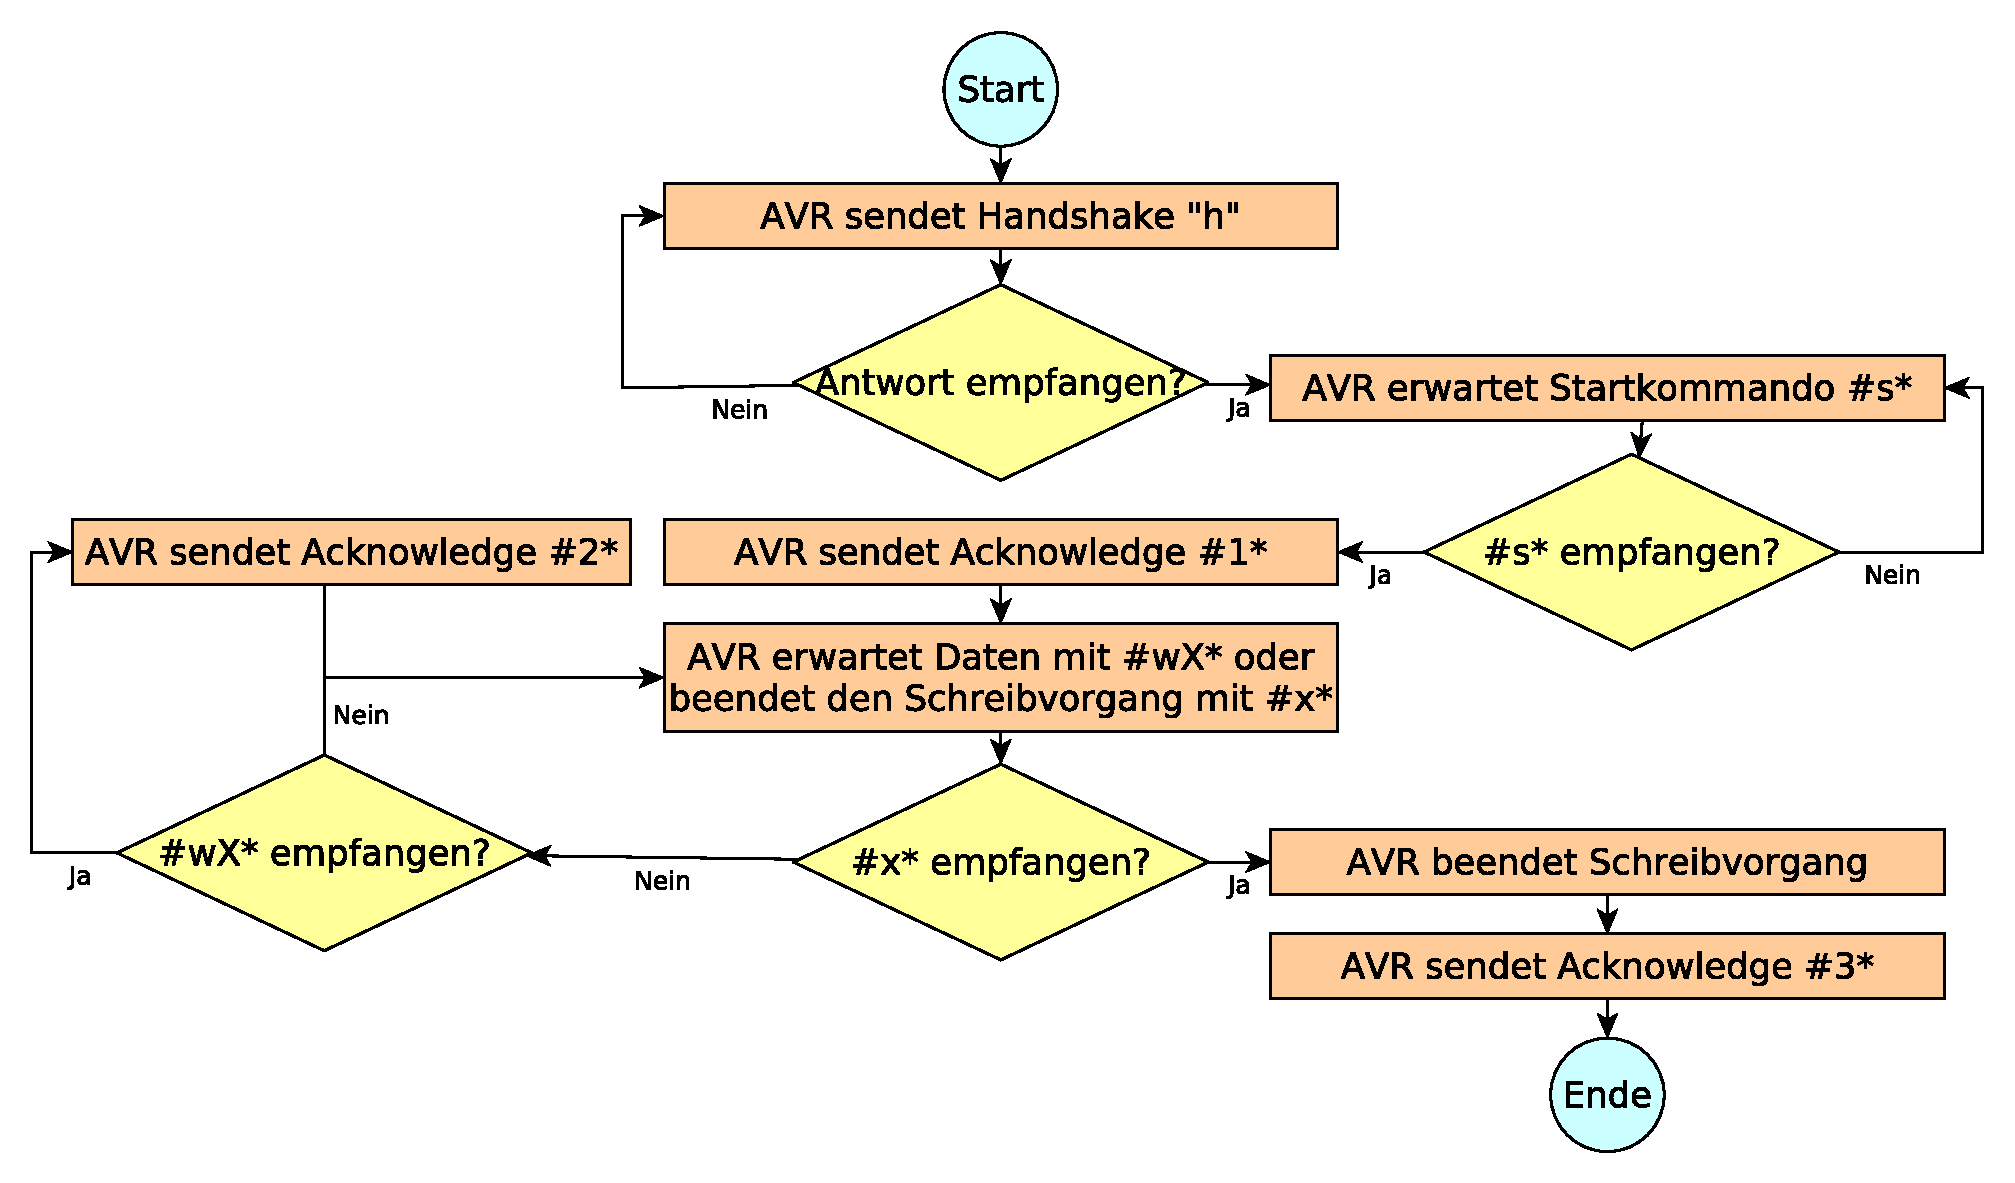
\includegraphics[width=1\textwidth]{TeilB/avr_arch.pdf}}
    \caption{Ablaufdiagramme Embedded-Software}
    \label{fig:ablaufdiagramm_avr} 
\end{figure}\\

Für den Fehlerfall, dass die Datenkommunikation abbricht, obwohl bereits das Startkommando \code{\#s\*} gesendet wurde, wird der Zyklus mit jedem erneuten Senden von \code{\#s\*} zurückgesetzt und der Schreibvorgang von vorne begonnen.\\
Wird die PC-Software gestartet und es bleibt das Handshake vom AVR aus (z. B. fehlerhafte oder falsche Software im AVR), so wird innerhalb einer Zeitspanne auf dieses Handshake gewartet und nach Ablauf dieser Zeit abgebrochen und der Fehler angezeigt.\\
Der gesamte Schreibvorgang ist innerhalb einer definierten Zeit abgeschlossen. Tritt im Fehlerfall eine Verzögerung auf, so wird ebenfalls nach Ablauf einer definierten Zeitspanne abgebrochen und der Fehler angezeigt.
\subsection{EDID-Daten auf Embedded-Seite}
In den folgenden Abschnitten wird auf die  internen Funktionsweisen und wichtiger Code-Ausschnitte der Embedded-Software eingegangen.\\
Wie bereits in \refc{softwarekonzept} angesprochen werden nach der Interpretation der Kommandos die entsprechenden Funktionen aufgerufen. Der AVR empfängt die Zeichen über die UART-Schnittstelle Zeichen für Zeichen. Wird ein Zeichen empfangen, wird ein Interrupt ausgelöst und dessen ISR\footnote{ISR: Interrupt Service Routine} aufgerufen. Der Quellcode der ISR ist in \refl{lst:uart_isr} gezeigt.
\begin{lstlisting}[%
language=MyC,
caption={Embedded-Software: UART-ISR},
label=lst:uart_isr
]
ISR(USART_RX_vect)
{
   sint8 next_char;
   next_char = UDR0;

   if(next_char == '#')
   {
      uart_str_cnt = 0;
      block_finished = 0;
   }
   if(next_char == '*' && !block_finished)
   {
      block_finished = 1;
      switch(uart_str[1])
      {
      case 's':
         command_ready(CMD_WRITE_START, 0xFF);
         break;
      case 'w':
         command_ready(CMD_WRITE_DATA, uart_str[2]);
         break;
      case 'x':
         command_ready(CMD_WRITE_STOP, 0xFF);
         break;
      case 'd':
         command_ready(CMD_DBG, 0xFF);
         break;
      case 'c':
         command_ready(CMD_CHECKSUM, 0xFF);
         break;
      case 'h':
         handshake_received = 1;
         break;
      default:
         command_ready(CMD_ERROR, 0xFF);
         break;
      }
   }
   if(!block_finished)
   {
      uart_str[uart_str_cnt] = next_char;
      uart_str_cnt++;
   }
}
\end{lstlisting}
Nach dem Empfang eines Zeichens im Register \code{UDR0} wird dieses in die Variable \code{next_char} gespeichert. Es wird innerhalb einer State-Machine überprüft, ob ein Kommando vollständig mit den Steuerzeichen \code{\#} und \code{\*} empfangen wurde. Solange das Flag \code{block_finished} nicht gesetzt ist, wird das aktuelle Zeichen an einen Buffer \code{uart_str[]} angehängt. Ist das Flag \code{block_finished} gesetzt und das aktuelle Zeichen entspricht \code{\*}, so ist das Kommando bereit interpretiert zu werden. Da das zweite Zeichen des Kommandostrings \code{uart_str[2]} jeweils den eigentlichen Kommandonamen definiert, reicht es diesen auszuwerten und die entsprechende Funktion mit \code{command_ready(uart_i2cCommandType cmd, uint8 data)} anzuspringen.
\refl{lst:eeprom_functions} zeigt die entsprechenden Funktionen für den Zugriff auf das EEPROM.\\
Die Funktion \code{w_start()} setzt internen Variablen auf deren Initialwerte zurück und beschreibt das Flag \code{connection_status}  mit \code{OPEN}.\\
Mit dem Aufruf der Methode \code{w_data(uint8 data)} werden die übergebenen Daten \code{data} an die aktuelle Stelle im EEPROM mit der Funktion \code{write_eeprom_byte(uint8 addresse, uint8 data)} an die Adresse \code{address_counter} geschrieben und der Adresszähler inkrementiert. Für die Prüfsummen-Berechnung wird, das empfangene Datum in das Array \code{cmds[]} an die entsprechende Stelle geschrieben.\\
Um die Übertragung abzuschließen wird der Funktionsaufruf \code{w_stop()} verwendet, welche alle Variablen wieder auf deren Initialwerte zurücksetzt.\\
Um das EEPROM für Testzwecke auslesen zu können, wird der Aufruf \code{dbg_output()} verwendet. Hier wird der Inhalt des EEPROMs direkt Adresse für Adresse ausgelesen und direkt ausgegeben.\\
Die Prüfsumme wird aus den im EEPROM befindlichen Datenwörtern von errechnet. Hierfür werden alle Elemente des EEPROMs ausgelesen und mit der logischen XOR-Verknüpfung miteinander verrechnet. Das Ergebnis wird als Prüfsumme zurückgesendet. 

\begin{lstlisting}[%
language=MyC,
caption={Embedded-Software: Funktionen zum Beschreiben des EEPROMs},
label=lst:eeprom_functions
]
void w_start()
{
   cnt = 0;
   address_counter = 0;
   connection_status = OPEN;    /* Leave connection open */
   _delay_ms(100);
   uart_puts("#1*");
}

void w_data(uint8 data)
{
   cmds[address_counter] = data;
   write_eeprom_byte(address_counter, data);
   address_counter++;
   _delay_ms(100);
   uart_puts("#2*");
}


void w_stop()
{
   address_counter = 0;
   connection_status = CLOSED;
   handshake_received = 0;
   _delay_ms(100);
   uart_puts("#3*");
}

void dbg_output()
{
   uint8 i;
   for(i = 0; i < 128; i++)
   {
      eeprom[i] = read_eeprom_byte(i);
      uart_putc(eeprom[i]);
   }
}

void send_checksum()
{
   uint8 i;
   checksum = 0;
   for(i = 0; i < 128; i++)
   {
      eeprom[i] = read_eeprom_byte(i);
      checksum ^= eeprom[i];
   }
   uart_putc(checksum);
}
\end{lstlisting}%
Um den Zugriff auf das EEPROM einfach zu gestalten, sind zwei API-Funktionen definiert. So stehen die Methoden \code{void write_eeprom_byte(uint16 address, uint8 data)} und \code{uint8 read_eeprom_byte(uint16 address)} zur Verfügung. Der Treiber basiert auf einem bereits existenten EEPROM-Treiber für Atmel AVR Prozessoren (siehe \cite{eeprom_lib}) und nutzt das $I^2C$-Hardwareinterface des Prozessors. \\
Die in der Hardware vorgesehene und in \refc{cha:sw_edid_daten} angesprochene Funktionalität zum Dimmen der Hintergrundbeleuchtung der Displays ist softwareseitig aus Zeitgründen in der Embedded-Software nicht realisiert. 
\subsection{EDID-Daten auf PC Seite}
Im vorhergehenden Abschnitt wurde bereits die notwendige Struktur zur Kommunikation behandelt. Nun wird hinsichtlich des PC-Programms das Konzept sowie wichtige Codestellen dargelegt. Das Programm ist in der Programmiersprache C und der Grafikbibliothek GTK+ \footnote{GTK: GIMP-Toolkit, \url{http://www.gtk.org}} entwickelt. Für das Anlegen des GUI-Layouts\footnote{GUI: Graphical User Interface, Grafische Benutzerumgebung} ist das Tool \code{glade}\footnote{\url{https://glade.gnome.org/}} in Verwendung. Zur Kommunikation ueber die serielle Schnittstelle (RS-232) wird ein bestehender  , unter GPL\footnote{GPL: General Public Licence} lizensierter, Treiber verwendet (siehe \cite{rs232_lib}).

Prinzipiell ist es möglich das EEPROM mittels einer seriellen Verbindung und einem Terminal-Emulator wie z. B. \code{picocom} oder \code{GNU screen} das EEPROM mit den entsprechenden Kommandos zu beschreiben. Damit dieser Prozess automatisiert und damit für den Anwender komfortabel wird, steht ein Programm namens \code{edid_writer} für Linux zur Verfügung. Das Programm kann die Verbindung zum AVR aufnehmen, den Handshake abarbeiten sowie die Programmierung des EEPROMs durchführen, indem es die eingelesenen EDID-Daten in die entsprechenden Kommandos für den Prozessor verpackt. Da die Kommunikation ungepuffert ist, muss das Programm jeweils auf die Antwort des AVRs für die entsprechenden Kommandos warten, bis erneute Daten gesendet werden dürfen. Die Parameter für die Kommunikation (serielles Device z. B. \code{/dev/ttyUSB0} und die Baudrate z. B. \code{9600}) werden in einer Konfigurationsdatei mit dem Pfad \code{\~/.edid_writer/config} gespeichert und beim Start des Programms ausgelesen. \refa{fig:edid_writer1} zeigt ein Bild des Programms, bei dem eine gültige EDID-Datei geladen ist. Diese wird dem Benutzer im HEX-Format angezeigt. 
\begin{figure}[htp]
	\center
	\fbox{	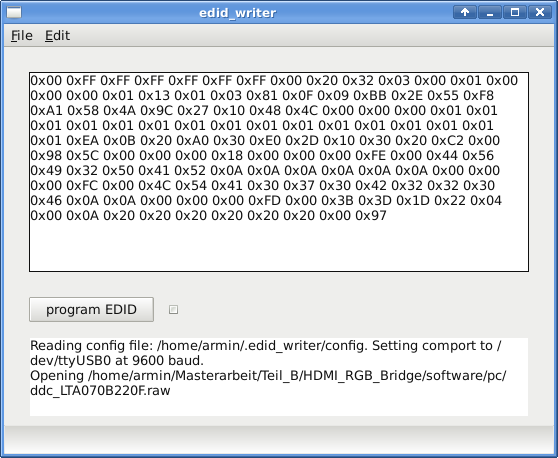
\includegraphics[width=0.6\textwidth]{TeilB/edid_writer1.png}}
    \caption{PC-Programm EDID-Writer}
    \label{fig:edid_writer1} 
\end{figure}\\
Um die Lesbarkeit der Codestücke zu verbessern, sind die Funktionsaufrufe der Grafikbibliothek \code{GTK+} entfernt, da diese nur der Visualisierung des Programms selbst dienen.\\
Um die EDID-Daten korrekt verarbeiten zu können, wird dieses beim Laden lesbar im Binär-Modus geöffnet, die Größe der Datei herausgefunden und ein entspreches großes Array \code{hexfile} vom Typ \code{hexfileType} angelegt. Der Datentyp enthält das Kommando selbst, Daten, der Erwartete Rückgabewert des Kommandos sowie ein Flag, das die Existenz von Daten anzeigt (z. B. bei \#wX\*). Der Datentyp \code{hexfileType} ist in \refl{lst:hexfileType} gezeigt.
\begin{lstlisting}[%
language=MyC,
caption={PC-Software: Datentyp hexfileType},
label=lst:hexfileType
]
typedef struct
{
   unsigned char cmd;
   unsigned char hex;
   unsigned char ack;
   unsigned char nodata_flag;
}hexfileType;
\end{lstlisting}%
Um Das Array \code{hexfile} zu befüllen wird die Datei zuerst Elementweise ausgelesen, die Ergebnisse in das Array \code{uint8 edid_raw[]} gespeichert und im Anschluss verteilt. Um das Protokoll einzuhalten, werden an die Kommandos mit den reinen Rohdaten der EDID-Datei die entsprechenden Kommandos für Start und Stop des Transfers (\code{\#s\*} und \code{\#x\*}) angefügt. Mit dem letzten Kommando wird die Prüfsumme abgefragt. Im Array \code{hexfile} befinden sich nach dem Laden also eine Liste von Elementen abzuarbeitender Kommandos. Zusätzlich wird beim Laden gleich die Prüfsumme berechnet. \refl{lst:hexfile_laden} zeigt den relevanten Codeausschnitt. 
\begin{lstlisting}[%
language=MyC,
caption={PC-Software: Hexfile Laden},
label=lst:hexfile_laden
]
hexfile = (hexfileType*)malloc((hexfile_size + CMD_C_SIZE + CMD_X_SIZE + CMD_S_SIZE) * sizeof(hexfileType));

   /* load the actual data into the program */
   for(cnt = 0; cnt < hexfile_size; cnt++)
   {
      edid_raw[cnt] = (0xFF & buffer[cnt]);
   }
   hexfile[0].cmd = 's';
   hexfile[0].hex = 0;
   hexfile[0].ack = '1';
   hexfile[0].nodata_flag = 1;

   for(cnt = 0; cnt < hexfile_size; cnt++)
   {
      hexfile[cnt+CMD_S_SIZE].cmd = 'w';
      hexfile[cnt+CMD_S_SIZE].hex = edid_raw[cnt];
      hexfile[cnt+CMD_S_SIZE].ack = '2';
      hexfile[cnt+CMD_S_SIZE].nodata_flag = 0;
      checksum ^= edid_raw[cnt];
   }

   hexfile[hexfile_size +  CMD_X_SIZE].cmd = 'x';
   hexfile[hexfile_size +  CMD_X_SIZE].hex = 0;
   hexfile[hexfile_size +  CMD_X_SIZE].ack = '3';
   hexfile[hexfile_size +  CMD_X_SIZE].nodata_flag = 1;

   hexfile[hexfile_size +  CMD_X_SIZE + CMD_C_SIZE].cmd = 'c';
   hexfile[hexfile_size +  CMD_X_SIZE + CMD_C_SIZE].hex = 0;
   hexfile[hexfile_size +  CMD_X_SIZE + CMD_C_SIZE].ack = '4';
   hexfile[hexfile_size +  CMD_X_SIZE + CMD_C_SIZE].nodata_flag = 1;
\end{lstlisting}%
Die eigentliche Hauptfunktion des Programms wird beim betätigen des Buttons zum Programmieren aufgerufen. Hier wird zuerst die serielle Verbindung aufgebaut. Im Fehlerfall wird eine Fehlermeldung ausgegeben. Ist der Verbindungsaufbau mit der korrekten Baudrate aufgebaut, wird abgefragt, ob das Handshake vom AVR empfangen wird. Wird dies nicht innerhalb einer Timeout-Zeitspanne empfangen, wird ebenfalls eine Fehlermeldung ausgegeben und abgebrochen. Die zu sendenden Kommandos aus dem Array \code{hexfile} werden mit die Funktion \code{char *returnSerialCommand(unsigned char cmd, unsigned char hex, unsigned char nodata_flag)} aufbereitet. Diese ist in \refl{lst:returnSerialCommand} zu sehen und gibt einen String mit dem entsprechenden Kommando zurück. 
\begin{lstlisting}[%
language=MyC,
caption={PC-Software: returnSerialCommand()},
label=lst:hexfile_laden
]
static char *returnSerialCommand(unsigned char cmd, unsigned char hex, unsigned char nodata_flag)
{
   char *buf;
   if(nodata_flag == 1){
      buf = (char*) malloc(sizeof(char) * 3);
      sprintf(buf, "#%c*", (char)cmd);
   }
   else{
      buf = (char*) malloc(sizeof(char) * 4);
      sprintf(buf, "#%c%c*", (char)cmd, (char)hex);
 buf[3]);
   }
   return buf;
}
\end{lstlisting}%
Innerhalb einer Maximaldauer, markiert mit \code{TIMEOUT_CYCLES}, findet das Senden komplett statt. Jedes Element des Arrays \code{hexfile} wird mit dem Index \code{command_index} durchlaufen und entsprechend mit der Funktion \code{returnSerialCommand} der zu sendende Kommandostring erzeugt und gesendet. Es wird auf Acknowledge vom AVR gewartet, bevor das nächste Kommando gesendet wird. Treten unerwartete Verzögerungen auf, so wird nach Ablauf der Timeout-Zeit eine Fehlermeldung ausgegeben und abgebrochen. \refl{lst:hexfile_schreiben} zeigt die Codestelle, mit der die Logik des Sendens realisiert ist. 
\begin{lstlisting}[%
language=MyC,
caption={PC-Software: Hexfile schreiben},
label=lst:hexfile_schreiben
]
 while (timeoutCounter < TIMEOUT_CYCLES) {
    if (command_sent == 0 && command_index <  hexfile_size + CMD_S_SIZE + CMD_X_SIZE + CMD_C_SIZE) {
        CMD_ACK = NO_ACK;
        waitForInterrupt = 0;

        command = returnSerialCommand(hexfile[command_index].cmd,
                  hexfile[command_index].hex,
                  hexfile[command_index].nodata_flag);
        rs232_puts(comport_fd, command, 4);

        waitForInterrupt = 1;
        command_sent = 1;
    }
    if (command_sent && new_data > 0) {
        if (new_data >= 2) {
            rs232_data_received();
        }
    }
    if (command_sent && CMD_ACK == ACK) {
        new_data = 0;
        CMD_ACK = NO_ACK;
        command_sent = 0;
        if (command_index < hexfile_size + CMD_S_SIZE + CMD_X_SIZE + CMD_C_SIZE) {
            command_index++;
        }
    }
    if (command_index >= hexfile_size + CMD_S_SIZE + CMD_X_SIZE + CMD_C_SIZE) {
        timeoutCounter = TIMEOUT_CYCLES + 1;
    }
    usleep(TIMEOUT_30MS);
    timeoutCounter++;
}
\end{lstlisting}%
\newpage
